\subsection{Mean model == Mean measurement?}
For a selection of three model measurements:

Over rheobase, input resistance, capacitance, and time constant, we took measurements by instancing two different models at  two different loctations in parameter space. With these two different models we took seperate measurements of all the appropriate model properties, then we averaged these measurements together, to get the 'mean measurements', secondly we created a 'mean model' by averaging the two points together in parameter space and instancing the 'mean parameter model'. We then used the mean model to create a third set of measurements.

When we have mean measurements, and also mean model measurements, it enables us to understand if bi-modal distributions of measurements in experimental data can pose a problem for optimization of cells.

We know from examining neuroelectro data closely that bi-modal distributions of input resistance, and cell membrane capacitance exist, but we do not always know how invalid it is to fit to the mean of a bi-modal distribution.

We expect the Izhikitich model, and the adaptive exponential models to support "regime" change, that is we know that there are regions in parameter space that where when entered cell behavior becomes fundamentally different. Some regions support tonic-bursting and other regions support chattering.

To verify that this may be a problem in real experiments, we set about establishing that it is a problem in modelling space.

\begin{figure}
    \centering
    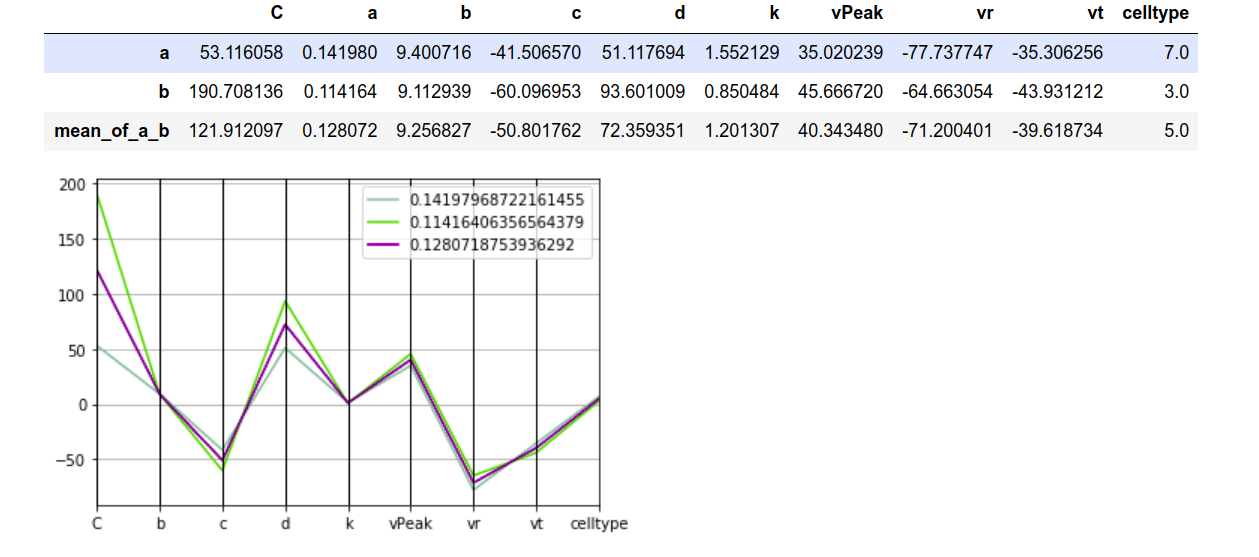
\includegraphics{figures/mean_model_mean_measure_ment_params.png}
    \caption{Caption}
    \label{fig:my_label}
\end{figure}

\begin{figure}
    \centering
    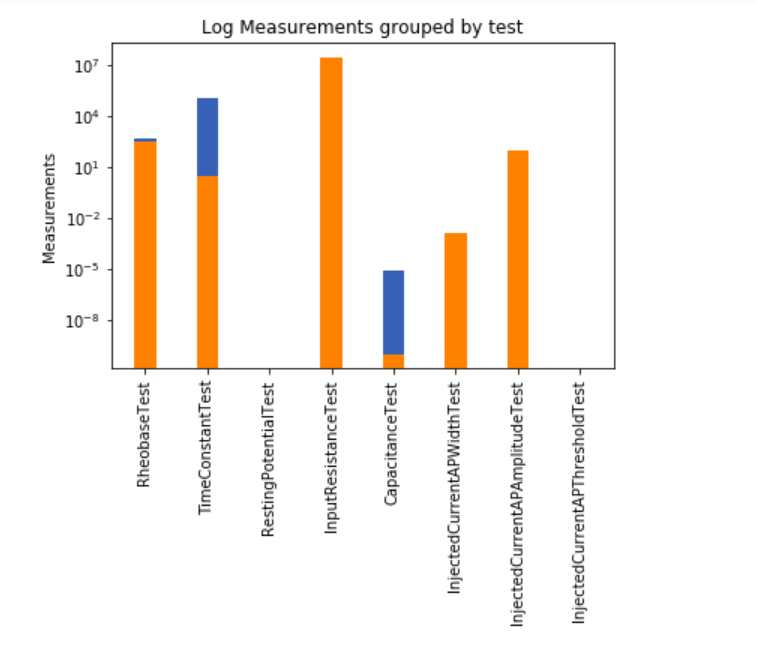
\includegraphics{figures/mean_model_mean_test.png}
    \caption{Caption}
    \label{fig:my_label}
\end{figure}

\begin{figure}
    \centering
    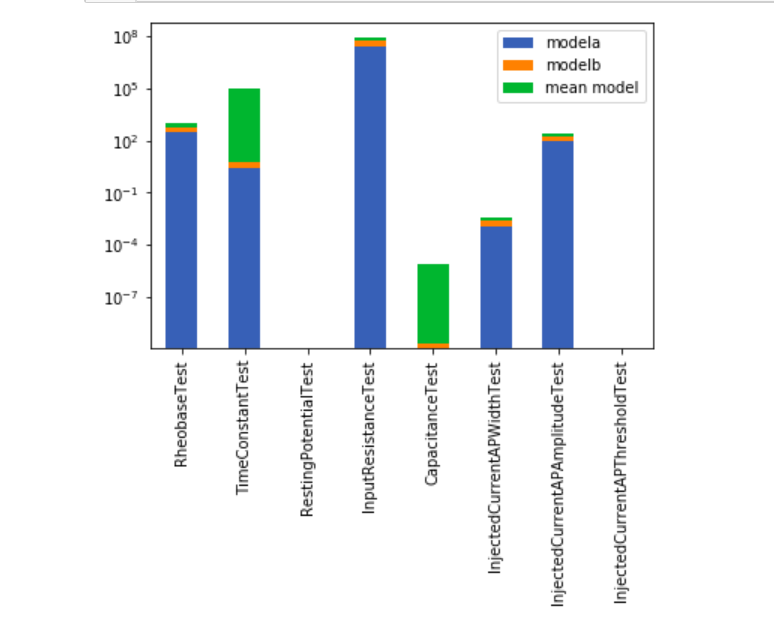
\includegraphics{figures/mean_model_mean_test2.png}
    \caption{Caption}
    \label{fig:my_label}
\end{figure}

explore if this was a problem for models as well as experimental cells.